% Created 2017-10-18 Wed 23:58
% Intended LaTeX compiler: pdflatex
\documentclass[titlepage]{article}
\usepackage[utf8]{inputenc}
\usepackage[T1]{fontenc}
\usepackage{graphicx}
\usepackage{grffile}
\usepackage{longtable}
\usepackage{wrapfig}
\usepackage{rotating}
\usepackage[normalem]{ulem}
\usepackage{amsmath}
\usepackage{textcomp}
\usepackage{amssymb}
\usepackage{capt-of}
\usepackage{hyperref}
\hypersetup{hidelinks=true}
\setlength{\parindent}{2em}
\usepackage[margin=1.2in]{geometry}
\author{Hu Xiaoxiang \\
U1521319A \\
EEE \\
}
\date{18 Oct, 2017 \\
}
\title{
\includegraphics[width=\textwidth]{logo_ntu_new.png} \\
[5\baselineskip] ASSIGNMENT \\
REPORT \\
[5\baselineskip]}
\hypersetup{
 pdfauthor={Hu Xiaoxiang \\
U1521319A \\
EEE \\
},
 pdftitle={
\includegraphics[width=\textwidth]{logo_ntu_new.png} \\
[5\baselineskip] ASSIGNMENT \\
REPORT \\
[5\baselineskip]},
 pdfkeywords={},
 pdfsubject={},
 pdfcreator={Emacs 25.1.1 (Org mode 9.1.2)}, 
 pdflang={English}}
\begin{document}

\maketitle
\tableofcontents

\pagenumbering{roman}
\newpage
\pagenumbering{arabic}

\section{Introduction}
\label{sec:orgc46124e}
\subsection{Background}
\label{sec:org31af3dd}
Equalization is the process of adjusting the balance between frequency
components within an electronic signal. An audio equalizer is an audio device
with multiple frequency controls for adjusting sound tone quality. To be
specific, an equalizer can be used to compensate for deficiencies in a sound
pickup or to reduce extraneous sounds, such as noise. Besides, it can also be
used to improve instrument clarity. For example, boosting a sounds harmonics
gives the impression of more presence and brightness and decresasing a sounds
harmonics gives the impression of a dull, less dazzling sound.
\subsection{Motivation}
\label{sec:org3a823db}
The audio output quality of loudspeakers may not be uniform due to size,
mechanical and cost constraints, even though they are usually designed to
have a fairly uniform response across the frequency spectrum. Therefore,
audio equalizer is performed to flatten this response, or to shape it
according to listener preferences.

In the early years, analog filters were mainly used to implement the audio
equalizer. However, the proliferation of digital audio sources, such as the
Internet and the USB, gives an opportunity to apply digital signal processing
to audio signals. Actually, many advantages, which include simplification of
design and verification, greater flexibility and reliability, and
significantly superior sound quality, allow the creation of digital equlizer
that can outperform its analog counterparts.
\subsection{Objective}
\label{sec:orgfac7921}
The objective of this project is to design and simulate an digital audio
equalizer using Matlab. It includes both implementation and evaluation of
the audio equalizer. 
\subsection{Report Outline}
\label{sec:orgadad803}
This report mainly constists of two parts: the implementation and the
performance analysis of an audio equalizer. In the implementation, the
procedure of creating a Graphical User Interface (GUI) by using Matlab's App
Designer and the construction of a FIR filter by using Matlab's DSP toolbox
is included. Meanwhile, the performance analysis focuses on displaying the
equalizer simulation result and elaborating the difference among outcomes
when different filter algorithms and configurations are applied.
\section{Design And System Construction}
\label{sec:org301db9d}
The entire audio equalizer consists of 3 major blocks: audio input, digital
audio equalizer and audio output. The audio input is implemented through
Matlab's internal audioread() function. The audio output, which includes the
DAC and reconstruction filter, is built on Matlab's sound() function.

\begin{center}
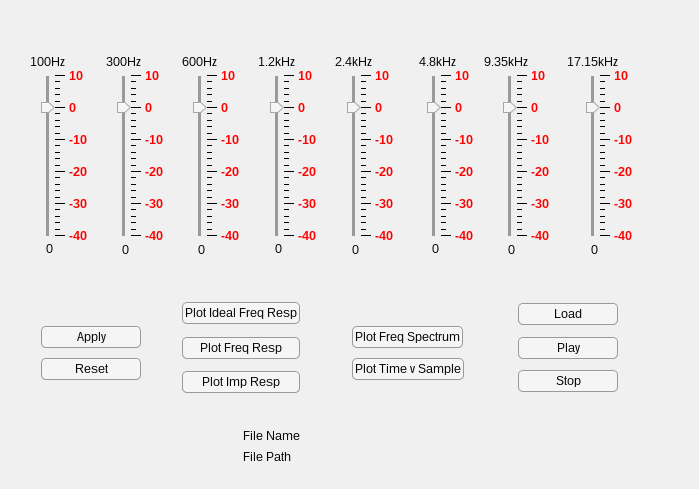
\includegraphics[width=.9\linewidth]{layout.png}
\end{center}

The GUI is designed by using Matlab's App Designer. As shown in the figure
above, each frequency band in the equalizer is controlled by a slider. The
'Apply' button collects the values set by sliders and pass to fir2() function
to generate the filters' coefficients b. The 5 'plot' buttons plot the figure
of the different response of the filter.
\section{Algorithm}
\label{sec:org5bcea8c}
The FIR filter function used in this equalizer is b=fir2(n,f,m,npt,lap,wind),
where n, f, m, npt, lab and wind represent filter order, frequency interval,
magnitude corresponding to each frequency interval, number of grid points,
length of region around duplicate frequency and window function. 

fir2() uses frequency sampling method to design FIR filter. The function
interpolates the desired frequency response linearly onto a dense, evenly
spaced grid of length npt, which is default set to 512. fir2 also sets up
regions of lap points around repeated values of f to provide steep but smooth
transitions. To obtain the filter coefficients, the function applies an
inverse fast Fourier transform to the grid and multiplies by window.

For example, to obtain the coefficients of a low pass filter like the figure
below, the function samples the desired frequency response of the filter and
then maps the sampling points to a grid. The number of sampling points depends
on the value of npt. lap, as shown in the second figure below, decides the
width between band edges. Less the value of lab, steeper the transitions from
edge to edge. The sampling points are stored in a vector and sent to inverse
fast Fourier transform function to get the filter coefficients b.

\begin{center}
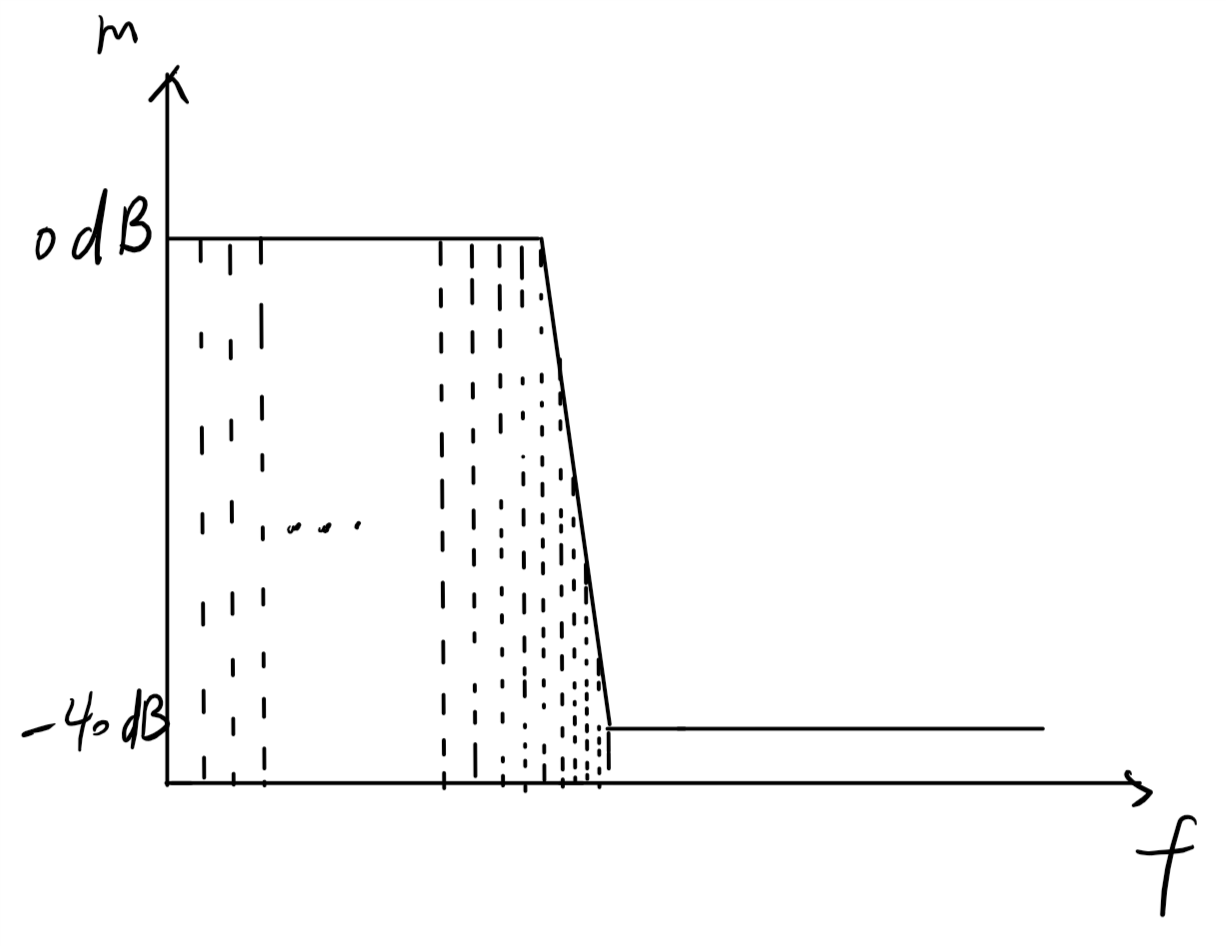
\includegraphics[width=.9\linewidth]{a.png}
\end{center}
\begin{center}
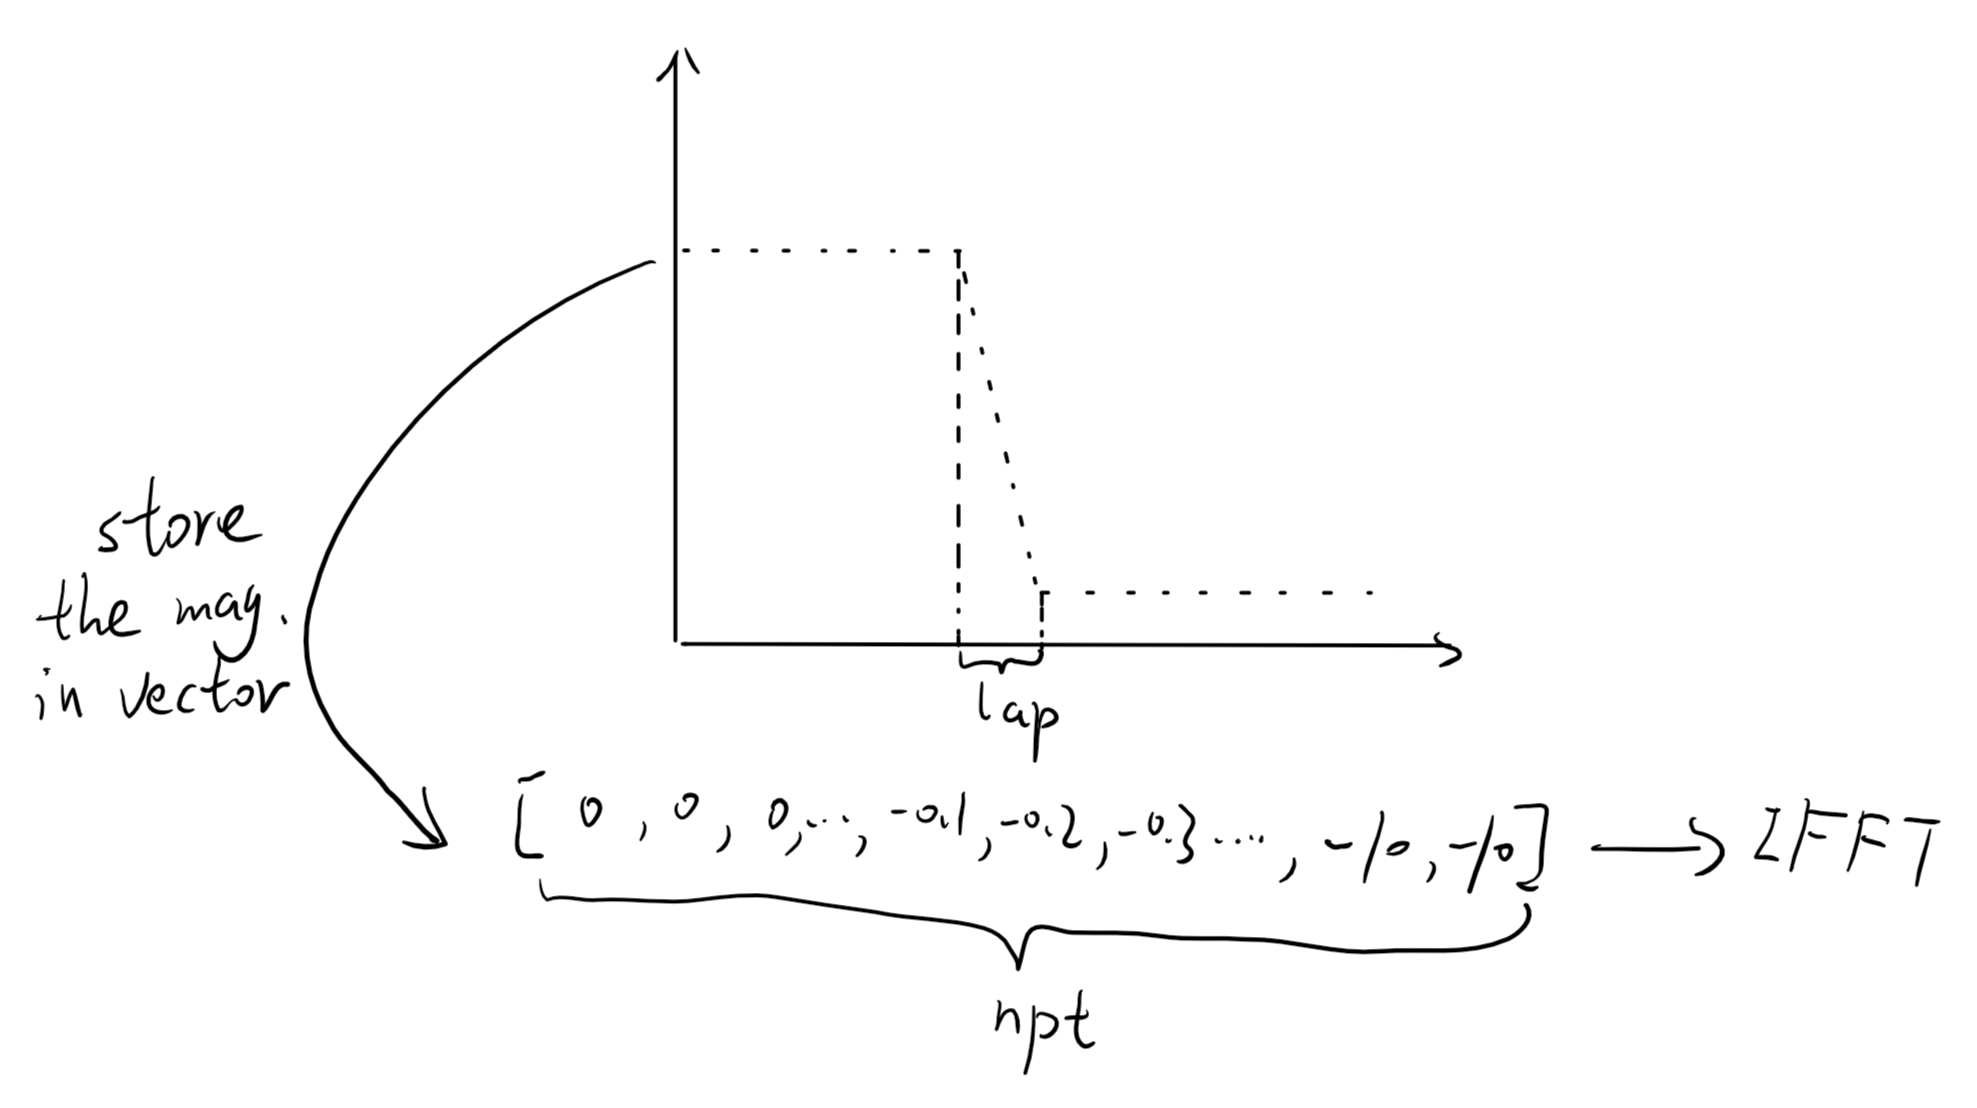
\includegraphics[width=.9\linewidth]{b.png}
\end{center}

\section{Results And Analysis}
\label{sec:orgc7ebd34}
\subsection{Results}
\label{sec:org4248f21}
Simulation setting: 

a) Signal components below 500 Hz and above 4000 Hz being
enhanced.

\begin{center}
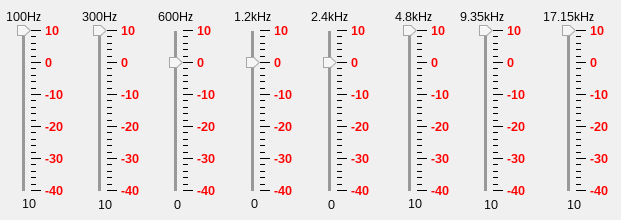
\includegraphics[width=.9\linewidth]{setting_a.png}
\end{center}

Ideal frequency response:

\begin{center}
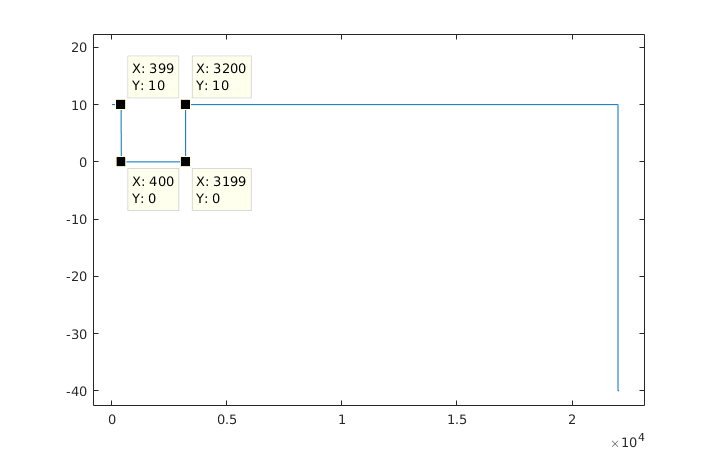
\includegraphics[width=.9\linewidth]{ideal_fr_a.png}
\end{center}

Actual frequency response:

\begin{center}
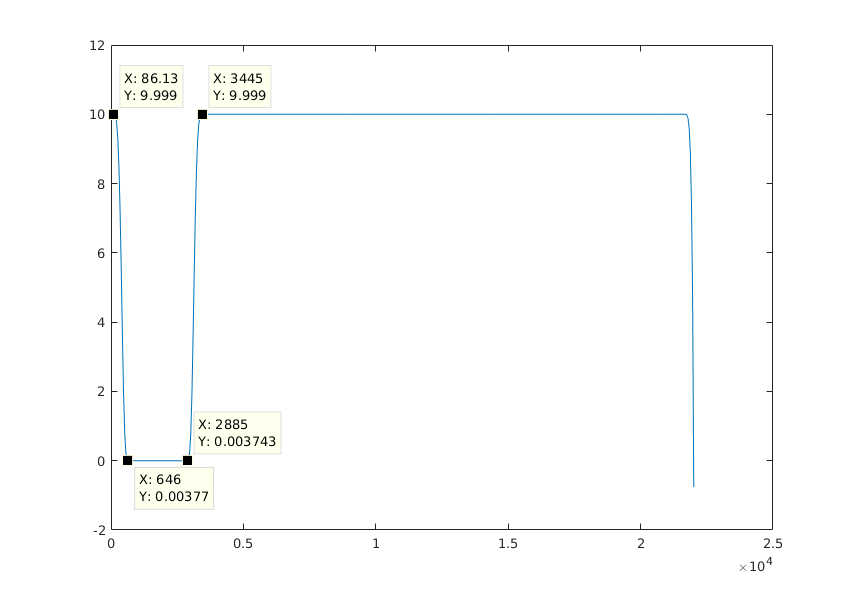
\includegraphics[width=.9\linewidth]{fr_a.png}
\end{center}

Impulse response:

\begin{center}
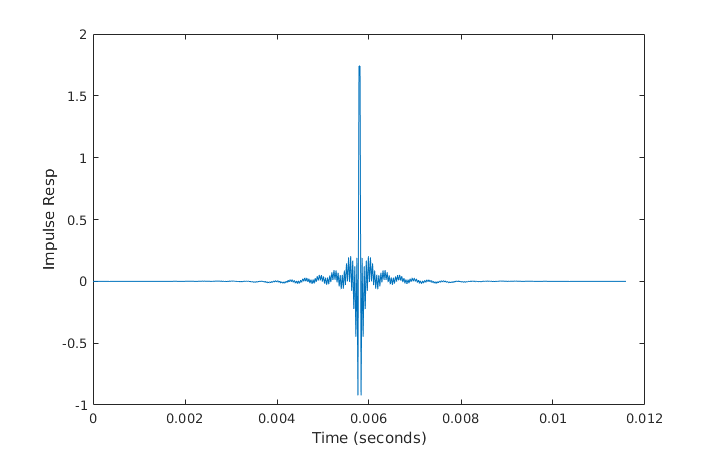
\includegraphics[width=.9\linewidth]{ir_a.png}
\end{center}

Frequency spectra:

\begin{center}
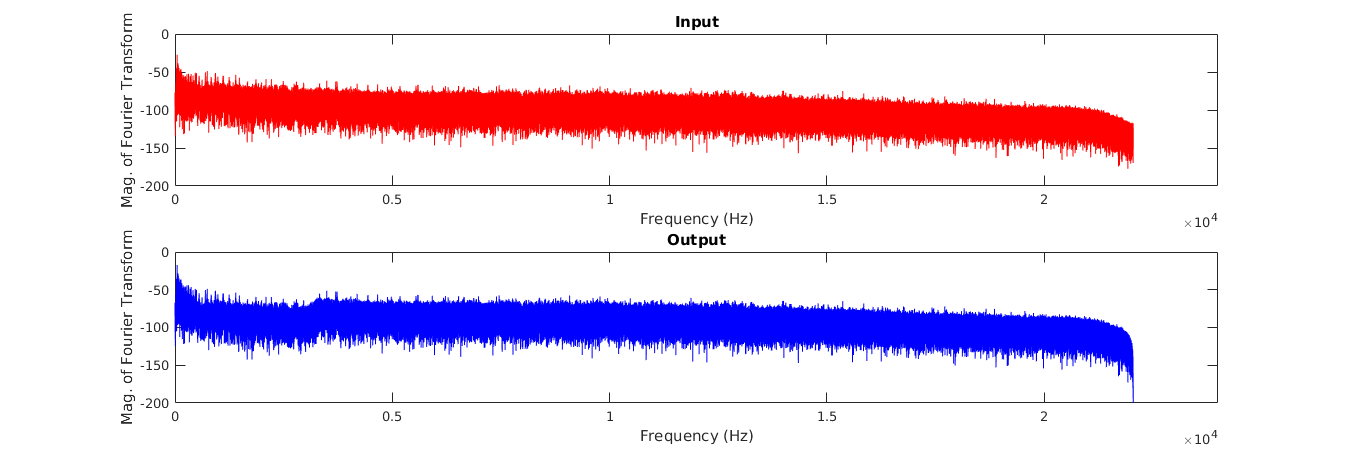
\includegraphics[width=.9\linewidth]{fs_a.png}
\end{center}

b) Signal components between 500 Hz and 4000 Hz being enhanced.

\begin{center}
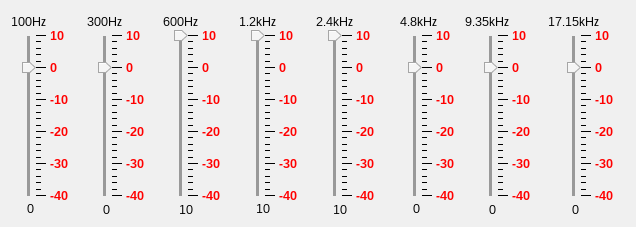
\includegraphics[width=.9\linewidth]{setting_b.png}
\end{center}

Ideal frequency response:

\begin{center}
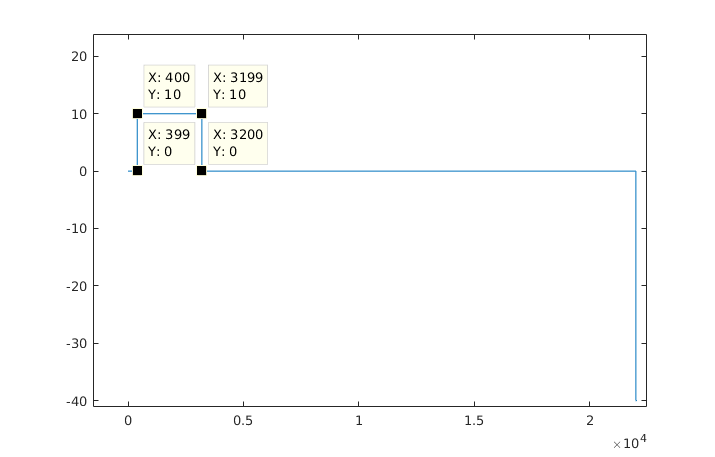
\includegraphics[width=.9\linewidth]{ideal_fr_b.png}
\end{center}

Actual frequency response:

\begin{center}
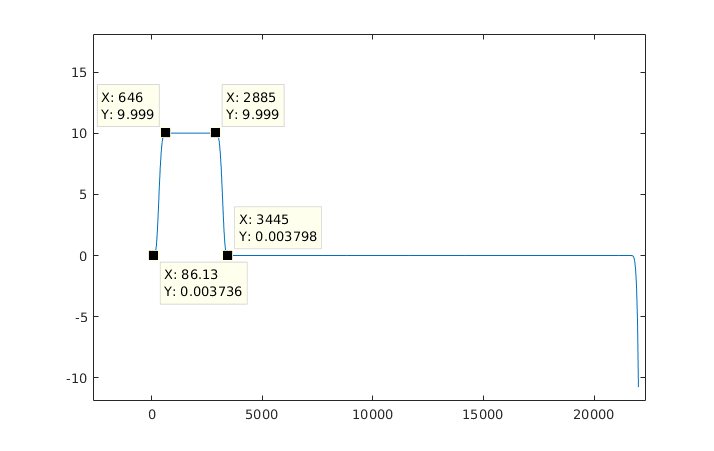
\includegraphics[width=.9\linewidth]{fr_b.png}
\end{center}

Impulse response:

\begin{center}
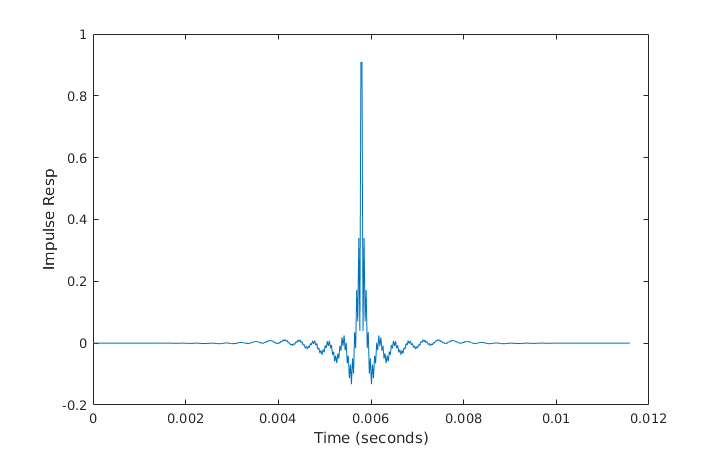
\includegraphics[width=.9\linewidth]{ir_b.png}
\end{center}

Frequency spectra:

\begin{center}
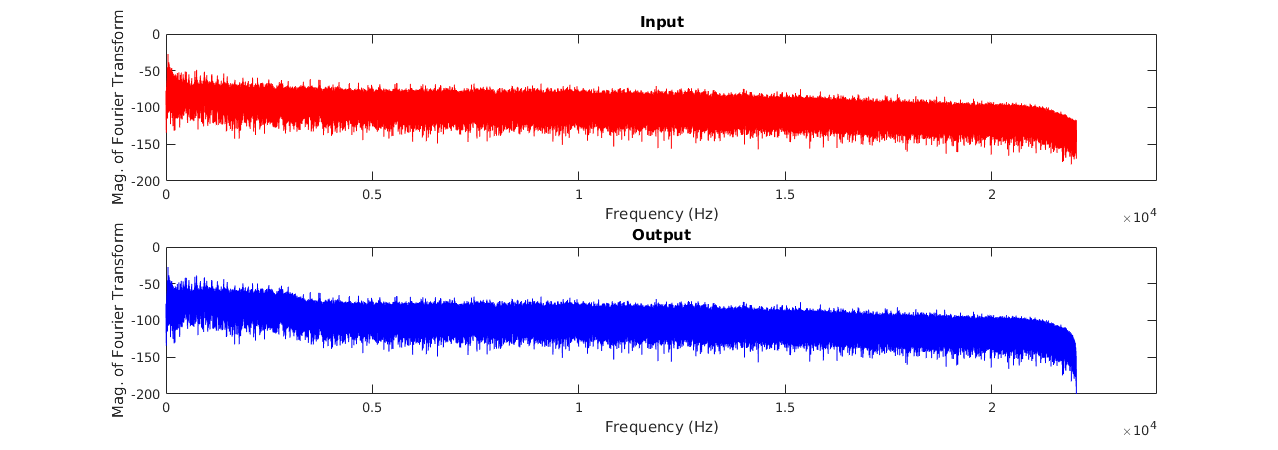
\includegraphics[width=.9\linewidth]{fs_b.png}
\end{center}

\subsection{Analysis}
\label{sec:orgea43428}
The figures above shows two different configurations of the equalizer. By
setting the gain of band 1,2,6,7,8 to +10dB, signal components below 400 Hz
and above 3200 are enhanced. On the second configuration, signal components
between 400 Hz and 3200 Hz are enhanced. 

As shown in the figure above, the transitions of an ideal filter frequency
response is steep. For actual frequency response, the transitions between
different band edges is more smooth. The transition band for setting a is
about 560 Hz and this is the main factor which limits the filter's
performance on low frequency band. For the bandwidth of low frequency band is
narrow, which is 200 Hz typically, a wide transition band can cause
significant influence on these section. One way to improve the performance is
to increase the filter order. The figure on below shows the frequency
response with 800 filter order.  the transition bandwidth now
decrease to around 300 Hz.

\begin{center}
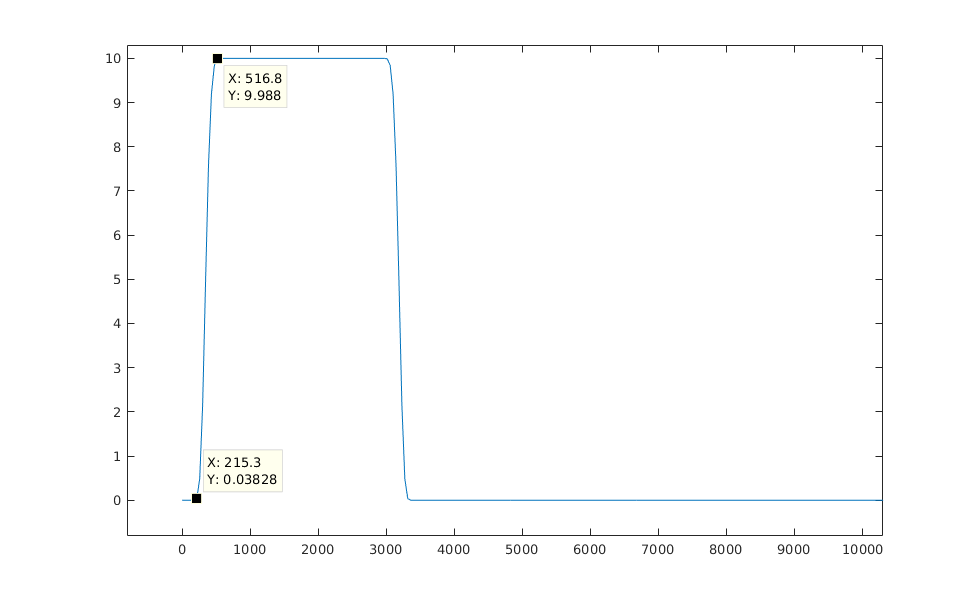
\includegraphics[width=.9\linewidth]{higher_order.png}
\end{center}

The obtained spectrum shows the result of the filtered signal. The shape of
the output spectrum corresponds to the shape of the FIR filter's frequency
response. 
\section{Conclusion And Recommendations}
\label{sec:orgbceac71}
In summary, the FIR filter basically meets the specification of an audio
equalizer. The result shows that the equalizer performs better on higher
frequency band compared to lower frequency band. Generally, the frequency
sampling method is a simple way to implement FIR filter. However, this method
requires longer filter length to achieve a more precise solution. In
comparison to other design method, such as window design method, least squared
method and the Parks-McClellan method, this method can have overall more
error. Thus, it is recommended to implement the digital equalizer by using
other method for a better solution on low frequency band.
\section{References}
\label{sec:orged80038}
\begin{enumerate}
\item Matlab Documentation 2017a
\end{enumerate}
\url{https://www.mathworks.com/help/signal/ref/fir2.html}

\begin{enumerate}
\item Wikipedia: Window Function
\end{enumerate}
\url{https://en.wikipedia.org/wiki/Window\_function}

\begin{enumerate}
\item StackExchange: Difference between frequency sampling and windowing method
\end{enumerate}
\url{https://dsp.stackexchange.com/questions/31905/}
difference-between-frequency-sampling-and-windowing-method
\end{document}
